\section{Observations}\label{section_two}
\begin{figure}[tbd]
\centering
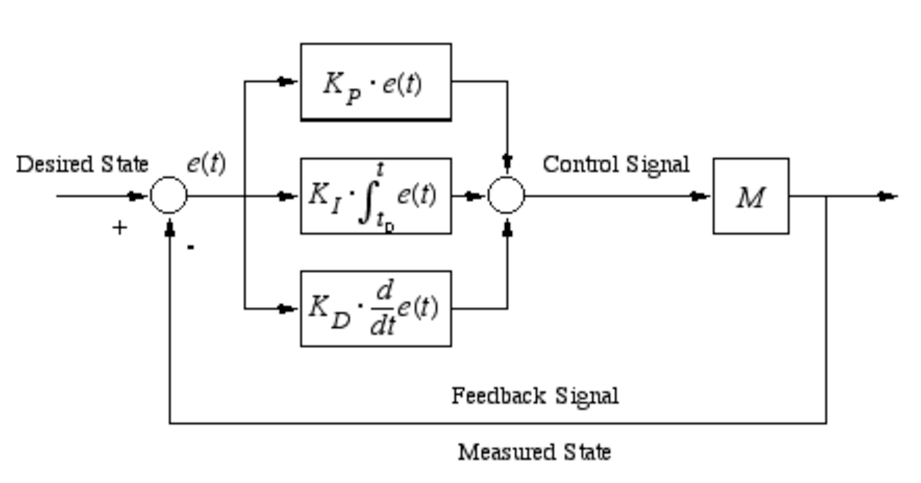
\includegraphics[width=0.5\textwidth]{images/pid.pdf}
\caption{\label{pid-controller} PID controller}
\end{figure}

\referenceFigure{pid-controller} represents a PID controller system\footnote{Image Source: \url{http://www.floatingvectors.com}}. As is shown by the diagram the difference between the ‘desired state’ and the ‘actual state’ (‘measured state’) is determined and calculated as the error of the system. This value is then processed by the PID controller and an output signal is sent to the device (often referred to as the Plant). The Plant then responds to the signal and using any sensors it is equipped with, produces a feedback signal dictating its new actual state. This cycle is looped until the desired state and the actual state functions are equivalent.
